\documentclass[10pt,conference]{IEEEtran}

% Set the margin
\usepackage{graphicx}
\usepackage{palatino}
\usepackage[scaled=0.92]{helvet}

\usepackage{url}
\usepackage{cite}
\usepackage{multicol}
\usepackage{listings}
\usepackage{color}
\usepackage{subfigure}
\usepackage{subfloat}
\usepackage{ifpdf}
\usepackage{epsfig}
\usepackage[ruled,vlined,linesnumbered]{algorithm2e}
\ExecuteOptions{letter}

\newcommand{\Cpp}{C\kern-0.05em\texttt{+\kern-0.03em+}}
\newcommand{\conceptCpp}{Concept\Cpp}

\newenvironment{commentenv}[1]{\begin{list}{}{}\item[]{\sc [#1:}
}{{\rm {\sc End of comment.]}} \end{list}}

%\long\gdef\comment#1#2{[\textsc{#1}: \textsf{#2}]}
\long\gdef\comment#1#2{}
\long\gdef\anju#1{\comment{Anju}{#1}}
\long\gdef\todo#1{\comment{To do}{#1}}

\newcommand{\code}[1]{\lstinline[basicstyle=\sffamily]{#1}}
\newcommand{\func}[1]{\lstinline[basicstyle=\sffamily]{#1()}}
\newcommand{\keyword}[1]{\emph{#1}}
\newcommand{\ConceptCpp}{ConceptC\kern-0.05em\texttt{+\kern-0.03em+}}
\newcommand{\MPIpp}{MPI\kern-0.05em\texttt{+\kern-0.03em+}}
\newcommand{\Cilkpp}{Cilk\kern-0.05em\texttt{+\kern-0.03em+}}
\newcommand{\Charmpp}{Charm\kern-0.05em\texttt{+\kern-0.03em+}}
\newcommand{\tablefont}{\fontsize{8}{15}\selectfont}
\renewcommand{\emph}{\textit}


\newcommand{\concept}[1]{{\sc #1}}

\lstdefinestyle{basic}{showstringspaces=false,columns=fullflexible,language=C++,escapechar=@,xleftmargin=1pc,%
basicstyle=\small\sffamily,
commentstyle=\mdseries,
moredelim=**[is][\color{white}]{~}{~},
morekeywords={concept,model,require,where,reduction,cilk,spawn,sync,omp,pragma,task,taskwait},
literate={->}{{$\rightarrow\;$}}1 {<-}{{$\leftarrow\;$}}1 {=>}{{$\Rightarrow\;$}}1,
}

\makeatletter

\renewenvironment{thebibliography}[1]
     {\section*{\refname
        \@mkboth{\MakeUppercase\refname}{\MakeUppercase\refname}}%
      \list{\@biblabel{\@arabic\c@enumiv}}%
           {\settowidth\labelwidth{\@biblabel{#1}}%
            \leftmargin\labelwidth
            \advance\leftmargin\labelsep
            \@openbib@code
            \usecounter{enumiv}%
            \let\p@enumiv\@empty
            \renewcommand\theenumiv{\@arabic\c@enumiv}}%
      \sloppy\clubpenalty4000\widowpenalty4000%
      \sfcode`\.\@m}
     {\def\@noitemerr
       {\@latex@warning{Empty `thebibliography' environment}}%
      \endlist}

\def\Box{{\ \vbox{\hrule\hbox{%                                            
   \vrule height1.3ex\hskip0.8ex\vrule}\hrule
  }}\par}

%%%%%%%%%%%%%%%%%%%%%%%%%%%%%%%%%%%%%%%%%%%%%%%%%%%%%%%
% A subfigure environment that can hold verbatim text %
%%%%%%%%%%%%%%%%%%%%%%%%%%%%%%%%%%%%%%%%%%%%%%%%%%%%%%%

\usepackage{subfigure}
\newbox\subfigbox
\makeatletter
\newenvironment{subfloat}%
{\def\caption##1{\gdef\subcapsave{\relax##1}}%
  \let\subcapsave\@empty%
  \setbox\subfigbox\hbox%
  \bgroup}%
{\egroup%
\subfigure[\subcapsave]{\box\subfigbox}}%
\makeatother

\lstset{language=C++,style=basic}

\usepackage{color}

\newcommand{\todoh}[1]{%
	\textcolor{green}{TODO: #1}
}

\newcommand{\todoa}[1]{%
	\textcolor{blue}{TODO: #1}
}

\newcommand{\insimgx}[3]{%
  \begin{figure}[!htbp]
  \begin{center}
    \includegraphics[width=#1]{./figs/#2}
    \caption{#3}
    \label{#2}
  \end{center}
  \end{figure}
}


\begin{document}
\title{Demand-driven Execution of Static Directed Acyclic Graphs 
       Using Task Parallelism}
\author{\IEEEauthorblockN{Prabhanjan Kambadur\IEEEauthorrefmark{1},
                          Anshul Gupta\IEEEauthorrefmark{2},
                          Torsten Hoefler\IEEEauthorrefmark{1} and
                          Andrew Lumsdaine\IEEEauthorrefmark{1}}
\IEEEauthorblockA{\IEEEauthorrefmark{1}Open Systems Lab, 
                                       Indiana University, 
                                       Bloomington, Indiana 47405.}
\IEEEauthorblockA{\IEEEauthorrefmark{2}IBM T. J. Watson Research Center, 
                                        Yorktown Heights, 
                                        New York 10598.}}
\date{}
\maketitle

\begin{abstract}
The dataflow model allows natural expression of parallelism in an application.
Applications expressed in the dataflow model can be executed either using the
data-driven or the demand-driven schemes. Although both these schemes have
their utility in different scenarios, the realization of the demand-driven
scheme is not adequately supported in the existing solutions for task
parallelism. In this paper, we examine some of the requirements placed by the
demand-driven execution scheme on task parallelism. We present PFunc, a new
library-based solution for task parallelism that fully supports the
demand-driven execution scheme. We compare the runtimes and peak memory
consumption of an unsymmetric sparse LU factorization emulation parallelized
using both the data- and demand-driven execution schemes. This comparison shows
that the demand-driven model provides benefits that necessitate its full
support in task parallelism.
\end{abstract}

\section{Introduction}
Program execution can often 
be modeled as the execution of a directed acyclic graph
(DAG) $G=(V,E)$ where the vertex set $V$ represents computations and the edge
set $E$ represents data dependencies (communications). Such \emph{dataflow}
schemes are an excellent means of expressing  application-level parallelism.
In particular, such DAG representation of computational problems facilitates
their parallelization and efficient execution using the \textit{task parallel}
programming paradigm.  In task parallelism, programs are divided into individual 
tasks and, subsequently, independent tasks are executed in parallel.

The dataflow model can be classified based on the order in which the
computations (vertices) encoded by the DAG are executed. In the
\textit{demand-driven} dataflow model, computations are initiated when there is
a demand for data.  Conversely, in the \textit{data-driven} dataflow model,
computations are initiated as and when those computations' inputs become
available.  Both the demand-driven and the data-driven models are important
programming paradigms of the dataflow model, and are suitable in different
scenarios.  Consider the execution of Algorithm~\ref{alg:fib} that calculates
the $N^{th}$ Fibonacci number. The algorithm functions by recursively dividing
the task of calculating the $N^{th}$ Fibonacci number (for $N \ge 2$), into the
tasks of calculating the $(N-1)^{st}$ and the $(N-2)^{nd}$ Fibonacci numbers.
In Algorithm~\ref{alg:fib}, new computations are initiated when there is a
demand for data and hence, it is an example of the demand-driven dataflow
model. One way of parallelizing Algorithm~\ref{alg:fib}'s execution is to
create a new task for each invocation. In the naive implementation of the
Fibonacci number calculator in this algorithm, the tasks of calculating the
$(N-1)^{st}$ and the $(N-2)^{nd}$ Fibonacci numbers are independent of one
another, and they can be executed in parallel.  Figure~\ref{fig:fibo} shows the
tree DAG that represents the execution of Algorithm~\ref{alg:fib} for $N=3$.
Notice that although Algorithm~\ref{alg:fib} can be expressed in the
data-driven dataflow model, the demand-driven model is a more natural way of
expressing this algorithm.

% Fibonacci Algorithm.
\begin{algorithm}[t]
\SetKwFunction{Fibonacci}{Fibonacci}

\caption{Fibonacci}
\label{alg:fib}

\KwIn{$N$}

\If{$N \le 1$}{
  return $N$;
}
return \Fibonacci{$N-1$} + \Fibonacci{$N-2$}
\end{algorithm}

\begin{figure}[b]
\begin{center}
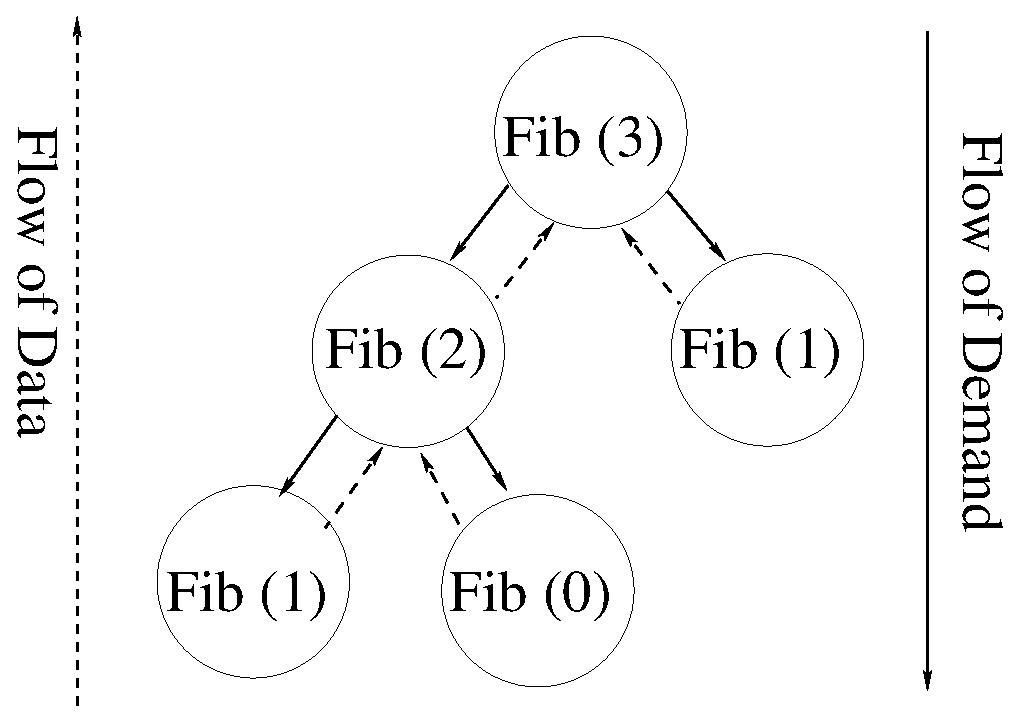
\includegraphics[width=0.32\textwidth]{figs/fib.eps}
\caption{Execution of Algorithm~\ref{alg:fib} with $N=3$.}
\label{fig:fibo}
\end{center}
\end{figure}

%
% Briefly state the problem and summarize the paper
%
Current solutions for task parallelism only support the demand-driven model
when executing tree DAGs. Therefore, although they suffice to parallelize
algorithms such as Algorithm~\ref{alg:fib}, they are insufficient to
parallelize algorithms that are encoded as general DAGs. However,
the current solutions for task parallelism fully support the data-driven
execution of general DAGs.
%
As a result, programmers who are unable to express their solutions
efficiently in a tree-based demand-driven scheme are forced to resort to
modeling their solutions using the data-driven dataflow model even though it
may be detrimental to their programming style and the application's overall
performance (runtime, memory footprint, or both). In this paper, we examine the
requirements placed by the demand-driven dataflow model on task parallelism,
and present a new solution for task parallelism, \textit{PFunc}, that supports
both the data- and demand-driven models efficiently.  We evaluate the
performance of both these models in executing general DAGs by emulating the
execution of a sparse unsymmetric LU factorization algorithm.  We characterize
performance  based on two parameters: speedup and memory footprint.  

\section{Background}
\label{sec:back}
Coarse-grained dataflow model is an excellent means of expressing
application-level parallelism.  Several functional languages and transformation
schemes for compilers, such as Arvind's Id~\cite{Arvind78},
Sisal~\cite{Feo1990}, LUSTRE~\cite{Caspi1987} and the
BLAZE~\cite{Mehrotra88programmingparallel} family of languages have been
proposed in order to generate efficient code for dataflow execution schemes.
%

Several groups have modeled linear algebra problems as dataflow DAGs. Kurzak
and Dongarra~\cite{kurzak08} implement dense linear algebra algorithms such as
LU, QR and Cholesky factorizations with this approach.  Sparse matrix
factorization is also often decomposed into DAG representation, and the
dataflow model is used to efficiently parallelize these DAGs on both shared-
and distributed-memory parallel
computers~\cite{GUPTA00wsmp2,GUPTAsimax01,HADFIELDthesis,DEMMEL97tr943}.
Although optimal scheduling of a DAG (both data- and demand-driven) is
NP-complete, heuristic approaches to DAG scheduling have been extensively
researched~\cite{KWOK99jpdc, KWOK99acm, GERAS92jpdc, SHIRAZI90jpdc}. It is
important to note that the focus of the current paper is on expositing the
requirements placed by the demand-driven execution of DAGs on existing
solutions for task parallelism.  Therefore, we are \textbf{not} concerned with
the problem of scheduling the execution of DAGs. Our approach is to execute
DAGs by spawning tasks when appropriate.  Therefore, the DAG scheduling problem
is reduced to one of task scheduling, which is handled by the task parallel
solution in use.

%
% Parallel solutions available
%
Many solutions have been implemented to facilitate dynamic task parallelism.
Fortran M~\cite{Foster97}, Cilk~\cite{FrigoLeRa98} and OpenMP
3.0~\cite{kn:omp_30} implement task parallelism as extensions to stock
programming languages. Other solutions such as Intel's Threading Building
Blocks (TBB)~\cite{kn:tbb}, Microsoft's Parallel Patterns Library (PPL) and
Task Parallel Library (TPL), and Java Concurrency Utilities are library-based.
All of the three HPCS languages (Chapel~\cite{Chamberlain:2007p1040},
Fortress~\cite{fortress} and X10~\cite{Charles:2005p1232}) offer task
parallelism as language features. Scheduling of tasks has received wide
attention in the programming community. Cilk's \textit{depth-first
work}~\cite{Blumofe94} model, the X10 Work Stealing framework's (XWS)
\textit{breadth-first}~\cite{Cong08} model and Guo et al's hybrid
model~\cite{Sarkar09} are notable examples of work-stealing schedulers.  All of
the three above mentioned schedulers implement variations of the
\textit{strict} computation model~\cite{Blumofe94} where each task returns to
exactly one ancestor. Consequently, the task spawn structure in all these
models is a tree DAG. 
% Futures
\textit{Futures}~\cite{Halstead85}  have been proposed as a means of exploiting
application-level parallelism. Although semantically different from tasks, futures offer many
of the same features as tasks.  In addition, futures can be passed around and
copied thereby allowing execution of general DAG structures. Notably, Cray XMT's
Programming Environment~\cite{cray} provides support for first-class futures.

\section{Parallel Execution of DAGs}
\label{sec:parallel} 
In this section, we take a closer look at strategies that help us realize the
data- and demand-driven models using task parallelism.  In particular, we look
at the requirements placed by these strategies on task parallelism and the
advantages and disadvantages of each strategy.  In the rest of this paper, we
use the terms ``node'' and ``task'' interchangeably. 

\subsection{Terminology}
\label{sec:terminology}
For the sake of clarity, we will first explain the DAG terminology that will be
used throughout the paper.  In the data-driven model, an edge $e=(u
\rightarrow{} v)$ in the DAG (dubbed the data-DAG) implies that $u$ is the
producer of the data consumed by $v$. Here, $u$ is called the data-parent and
$v$ the data-child.  A node in the data-DAG that has no incoming edges is
called a data-root. Data-roots represent nodes that have no data dependencies.
Similarly, a node that has no outgoing edges is called a data-leaf. 
%
Alternately, in the demand-driven model, an edge $e=(u \rightarrow{} v)$ in the
DAG (dubbed the demand-DAG) implies that $u$ is the consumer of the data
produced by $v$. Here, $u$ is called the demand-parent and $v$ the
demand-child. A node in the demand-DAG that has no incoming edges is called a
demand-root and a node that has no outgoing edges is called a demand-leaf.
Demand-leaves represent nodes that have no data dependencies and hence, no
demands.
%
It is easy to see that the data-DAG is the same as the demand-DAG, but with the
directions of all its edges reversed.  Therefore, demand-roots and
demand-leaves in a demand-DAG correspond one-to-one to the data-leaves and
data-roots respectively in the corresponding data-DAG.  For example, in
Figure~\ref{fig:fibo}, the data-DAG is represented with dashed edges and the
corresponding demand-DAG with solid edges. 

\subsection{Data-driven Execution of DAGs}
The basic premise of the data-driven execution model is to spawn new tasks upon
availability of data.  We can execute the data-DAG in this model by utilizing 
topological sort.  To achieve this, each node has its reference count
initialized to its indegree. Nodes that have a reference count of $0$ (require
no input) serve as the data-roots for the data-DAG's execution.  As each
node executes, it decrements the reference count of all its data-children. If
the reference count of any of its data-children goes to $0$, it implies that
this particular data-child has no unsatisfied dependencies and is immediately
spawned.  This strategy effectively induces a tree on top of the data-DAG where
each node has a \textit{spawning parent}.  This strategy is illustrated in
Algorithm~\ref{alg:data}, and is similar to the macro dataflow scheme presented
by Sarkar~\cite{Sarkar89}.  Lines $10, 11$ and $12$ of Algorithm~\ref{alg:data}
are required as Algorithm~\ref{alg:data} is written in the style of Cilk's
\textit{fully-strict} model where each node can only join its spawning parent.

\begin{algorithm}[t]

\SetKwFunction{Child}{Child}
\SetKwFunction{DataExecuteNode}{DataExecuteNode}
\SetKwFunction{Compute}{Compute}
\SetKwFunction{Wait}{Wait}
\SetKwFunction{OutEdges}{OutEdges}
\SetKwFunction{InEdges}{InEdges}
\SetKwFunction{Running}{Running}
\SetKwFunction{Spawn}{Spawn}

\caption{DataExecuteNode}
\label{alg:data}

\KwIn{A vertex $v$, data-DAG $G$}

\emph{/*Phase 1: Compute the results*/}\;
\Compute{$v$} \;

\emph{/*Phase 2: Iterate over each data-child and spawn eligible ones*/}\;
$SpawnedByMe \leftarrow \emptyset$\;
\ForEach{$e = (v \rightarrow{} c) \in$ \OutEdges{$v,G$}}{
  $RefCount[c] \leftarrow RefCount[c] - 1$\;
  \If{$RefCount[c] \equiv 0$}{
    \Spawn{\DataExecuteNode{$c,G$}}\;
    $SpawnedByMe \leftarrow SpawnedByMe \bigcup \{c\}$\;
  }
}

\emph{/*Wait for the data-children I spawned*/}\;
\ForEach{$c \in SpawnedByMe$}{
  \Wait{$c$}\;
}
\end{algorithm}

\subsubsection{Advantages}
As Algorithm~\ref{alg:data} induces a tree structure on the data-DAG, it can be
implemented using existing solutions for task parallelism.  Also, as all nodes
in the data-DAG are spawned as tasks, the user is not burdened with designing
an efficient scheduling strategy to execute the data-DAG. Instead, efficient
execution of the data-DAG now depends on smart scheduling of tasks. In this
regard, scheduling policies of existing task parallel solutions (see
Section~\ref{sec:back}) provide excellent support.

\subsubsection{Disadvantages}
In applications such as the sparse unsymmetric LU factorization described in
Section~\ref{sec:lu}, each node in the data-DAG produces data that lingers
until it is consumed by that particular node's data-children.  However, as each
data-child may have multiple data-parents, it cannot be launched until all its
data-parents complete.  Therefore, from a node's point of view, the lifetime of
its data depends on the structure of the data-DAG and the scheduling policy of
the tasking library in use.  Thus, the memory footprint of the application run
might be much larger than the optimal memory footprint for that particular run.
%
Furthermore, the data-DAGs produced in sparse LU factorization have a
significant number of computationally light data-roots.  Ideally, these
data-roots  should be executed sequentially as the task creation overhead is
substantial when compared to the computation time.  However, the data-driven
model disallows such decomposition of the problem.

%
% Discuss why we want all pieces of data to be available.
%
In Algorithm~\ref{alg:data}, a new node is not spawned until \textit{all} its
inputs become available. Alternately, if the application benefits from partial
computation, nodes can be spawned as soon as some of their inputs become
available. However, this strategy requires the nodes to block when more input
is required.  This has two disadvantages.  
%
First, note that a node can either allocate its required memory in chunks as
its inputs become available or allocate all of its required memory in one go.
When memory is allocated in chunks, application performance can degrade due to
the overhead involved in allocating memory in a parallel environment. When
memory is allocated upfront and, at one go, the node holds on to memory longer than
necessary. This in turn increases the memory footprint of the application.
%
Second,  the current solutions for task parallelism allow tasks to wait only on
their spawned descendants. No support exists for nodes to block on events other
than child completions. As such blocking is necessary for partial computation,
programmers will have to resort to external means of blocking such as OS
semaphores, thereby blocking whole threads instead of a single task.

\subsection{Demand-driven Execution of DAGs} 
The Fibonacci example in Algorithm~\ref{alg:fib} introduced the notion of
demand-driven execution. Algorithm~\ref{alg:demand} builds on this example and
presents a generic solution for executing demand-DAGs using task parallelism.
%
We begin execution starting with all nodes that have an indegree of $0$ in the
demand-DAG (i.e., the demand-roots). Each executing node first checks if each
of its demand-children have been spawned. If any of its demand-children are yet
unspawned, the node proceeds to spawn these demand-children. As a result, the
first demand-parent to reach a particular node is responsible for spawning that
node.  However, \emph{all} the demand-parents of every node wait on its
completion. Once all the demand-children of a node have finished executing, it
proceeds to execute its computations. Although each node has only one spawning
parent, notification of its completion is delivered to all its demand-parents.
Hence, Algorithm~\ref{alg:demand} does not impose a tree structure on the
demand-DAG.
%
\begin{algorithm}[t]

\SetKwFunction{Child}{Child}
\SetKwFunction{DemandExecuteNode}{DemandExecuteNode}
\SetKwFunction{Compute}{Compute}
\SetKwFunction{Wait}{Wait}
\SetKwFunction{Spawned}{Spawned}
\SetKwFunction{Spawn}{Spawn}
\SetKwFunction{OutEdges}{OutEdges}

\caption{DemandExecuteNode}
\label{alg:demand}

\KwIn{A vertex $v$, demand-DAG $G$}

\emph{/*Phase 1: Iterate over all demand-children and spawn unspawned ones*/}\;
\ForEach{$e = (v \rightarrow{} c) \in$ \OutEdges{$v,G$}}{
  \If{$\neg$ \Spawned{$c$}}{
    \Spawn{\DemandExecuteNode{$c$}}\;
  }
}

\emph{/*Wait for all the demand-children to complete execution*/}\;
\ForEach{$e = (v \rightarrow{} c) \in$ \OutEdges{$v,G$}}{
  \Wait{$c$}\;
}

\emph{/*Phase 2: Compute the results*/}\;
\Compute{$v$} \;
\end{algorithm}

\subsubsection{Advantages}
In the demand-driven model, a node is executed only when one of its
demand-parents is ready to consume the data that this node will produce.
Consequently, the data produced is used immediately. Furthermore, if all the
demand-parents of a particular node are ready to consume the data produced
(trivially true when the node has just one demand-parent), we can effectively
reduce the lifetime of the produced data, that is, the application's memory
footprint.
 
Demand-DAGs produced in many applications, such as factoring sparse matrices,
typically have just one demand-root.  This facilitates recursive partitioning
of the compute resources, and thereby, we can design custom scheduling
strategies that have better memory and speedup profiles than the data-driven
model. For example, in sparse matrix factorization demand-DAGs, nodes closer to
the demand-root are computationally heavier than the nodes closer to the
demand-leaves. In such cases, recursive partitioning helps users to employ data
parallelism in addition to task parallelism closer to the demand-root, and to
turn off task parallelism at a suitable distance from the demand-root
or at a suitable task granularity.
% An example for DAG
\begin{figure}[h]
\begin{center}
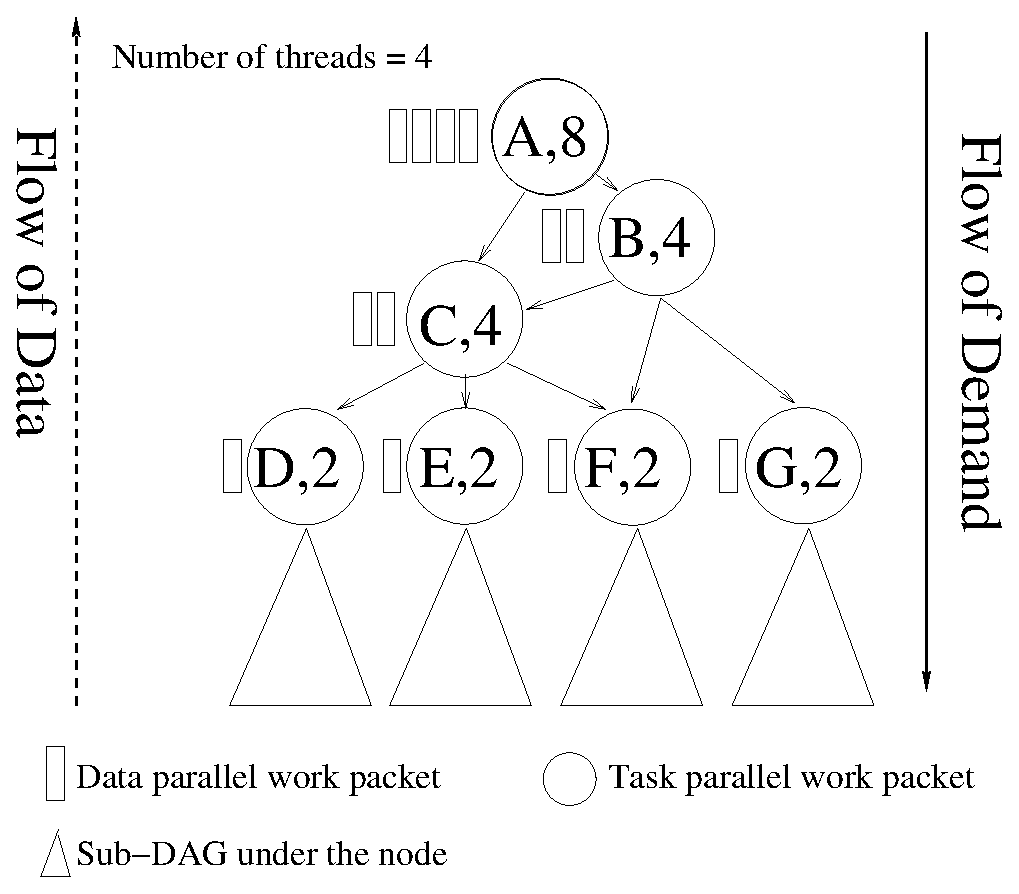
\includegraphics[width=0.40\textwidth]{figs/dag.eps}
\caption{Parallelization of a sample demand-DAG using both task and
         data parallelism. Each node is represented by an ID and 
         computational weight.}
\label{fig:dag}
\end{center}
\end{figure}

For example, consider the demand-DAG in Figure~\ref{fig:dag}. Each node in this
demand-DAG is represented by an ID and a number, which represents the weight of
the computation associated with that node (eg., node A has a computational
weight of 8). The areas represented as triangles represent sub-DAGs that are
rooted under the respective nodes.  Consider the execution of this sample
demand-DAG according to Algorithm~\ref{alg:demand} with 4 threads.  To
summarize, in \textit{Phase 1}, each node spawns all its unspawned
demand-children and waits on the completion of all the demand-children. Then,
in \textit{Phase 2}, each node proceeds to execute its local computations. This
algorithm can be optimized by being cognizant of the number of threads
available to each node for parallelizing its local computations.  For example,
as node A is the demand-root, it can utilize all 4 threads to execute its
computations in a data-parallel fashion.  Also, as nodes B and C have equal
computational weight, they are assigned 2 threads each, which they can use for
data parallel execution of their computations. In Figure~\ref{fig:dag}, the
number of threads assigned to each node and hence, the data parallelism at each
node is represented by rectangles to the left of each node.  Apart from data
parallelism, such recursive assignment of threads to each node can be used to
eliminate unwanted overhead of task creation at the lower levels. For example,
nodes D, E, F and G all have just one thread assigned to them. Therefore,
instead of spawning tasks to compute their demand-children, these nodes proceed
to execute their yet unspawned demand-children in a serial fashion. This
saves unnecessary task creation overhead for the nodes represented by the
triangles in Figure~\ref{fig:dag}.

\subsubsection{Disadvantages}
Although the demand-driven model allows more flexibility for custom scheduling
strategies, load balancing demand-DAG execution is in itself a hard problem
(see Section~\ref{sec:back}).  Furthermore, the demand-driven model cannot be
readily implemented using the existing solutions for task parallelism such as
Cilk, OpenMP, TBB and PPL. The issues that prevent the demand-driven model from
being implemented efficiently in the existing task parallel models are
discussed in the next section.

%
\begin{figure}[t]
\begin{center}
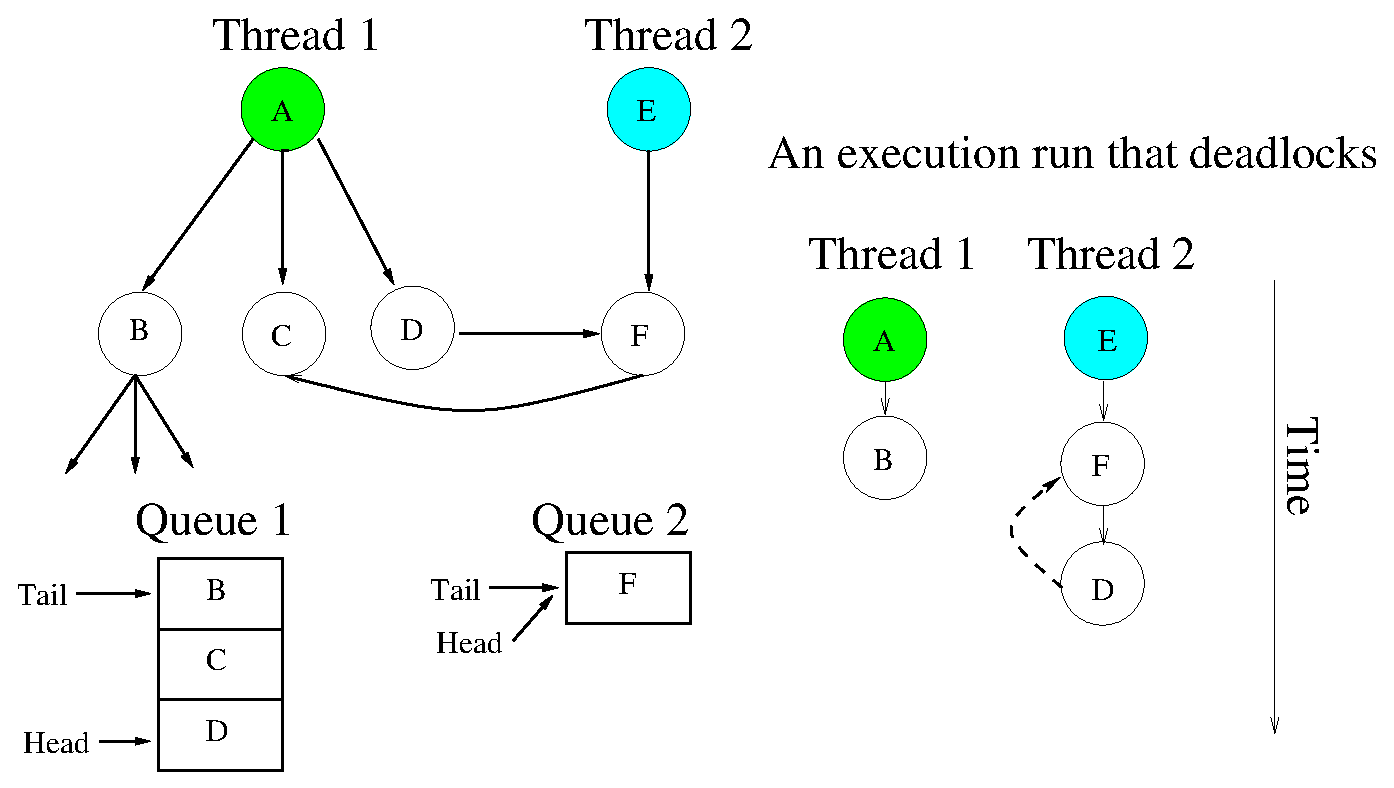
\includegraphics[width=0.50\textwidth]{figs/deadlock.eps}
\caption{A sample demand-DAG that can deadlock.}
\label{fig:deadlock}
\end{center}
\end{figure}

\subsection{Requirements of demand-driven model on task parallelism}
\label{sec:requirements}
In this section, we describe two of the requirements placed by the
demand-driven model on task parallelism. The second requirement is not met by
any of the existing tasking solutions.

\subsubsection{Continuations}
\label{sec:cont}
Algorithm~\ref{alg:demand} has two distinct phases. In \textit{Phase 1}, each
task spawns all its unspawned demand-children and waits on their completion. In
\textit{Phase 2} the local computations are performed. In order to efficiently
and correctly execute a demand-DAG thus, it is necessary to suspend the
execution of a task at the end of \textit{Phase 1} until all its dependencies
are satisfied. Such task suspension frees the thread executing this task to
perform other useful work. In other words, the tasking library should support
the execution of \textit{Phase 2} as a continuation of \textit{Phase 1}.  For
example, let us consider execution of the demand-DAG shown in
Figure~\ref{fig:deadlock} using Cilk's scheduling algorithm. In this example,
thread $1$ has tasks $B,C,D$ in its queue and thread $2$ has task $F$ in its
queue. thread $1$ executes task $B$ and thread $2$ executes task $F$.
Furthermore, assume that task $B$ gives rise to subsequent tasks that keep
thread $1$ busy.  As task $F$ waits for task $C$ to complete, it is free to
execute other tasks. In our case, as there are no more tasks in thread $2$'s
queue, thread $2$ steals and starts executing task $D$.  Depending on how task
$F$ was suspended in waiting for task $C$ to complete, two outcomes are
possible. First, if continuations are supported, task $D$ is suspended in wait
for task $F$. thread $2$ is then free to pick up task $C$ and complete its
execution. At this point, task $F$ can be completed and subsequently, task
$D$.  Second, if task suspension is implemented as a function call from
within the \func{Wait} call (see Algorithms~\ref{alg:data}
and~\ref{alg:demand}), when thread $2$ steals task $D$, it results in a
cyclic dependence between tasks $D$ and $F$, thereby resulting in a deadlock.
In Section~\ref{sec:lu}, we present an alternative scheme involving task
priorities and custom scheduling strategy that avoids such deadlocks.

% Current support for continuations
Cilk partially supports continuations through its \code{inlet} primitive.
OpenMP specifications mention that tasks can be suspended at either
pre-specified points (\code{tied} tasks) or at arbitrary points (\code{untied}
tasks) during their execution.  TBB supports the explicit continuation passing
style (CPS)~\cite{OliverCPS} of programming. 

\subsubsection{Multiple Completion Notifications}
In the demand-driven model, when a task completes, \textit{all} its
demand-parents should be notified so that they can consume the data that is
produced by this particular task. This requires that the tasking solution
support the delivery of multiple completion notifications. 
% Mention this is not available in any Cilk-like solutions.
However,  none of the existing tasking solutions support this feature.
Furthermore, in popular solutions for task parallelism such as Cilk, TBB,
OpenMP and X10, it is non-trivial to extend support for multiple completion
notifications as adherence to the strict computation model~\cite{Blumofe94} is
built into their schedulers.  In order to incorporate support for multiple task
completion notifications in these solutions, it would be necessary to modify 
their scheduling policies, which is non-trivial.
% Now, harp on this a bit more.
Support for multiple notifications is a hard requirement without which, the
correctness and the efficiency of the demand-driven model is compromised.  One
can remedy the lack of multiple notification support by resorting to using
system-level synchronization constructs such as locks and condition variables
to provide application-level notifications. However, these constructs operate
at the scope of threads and not tasks, and so, they block the entire thread
instead of just a single task.  When multiple notifications are supported by
the tasking library itself, while waiting for a task to complete, the parent
task is free to select and execute another task from the list of runnable
tasks.

\section{PFunc: A new tool for task parallelism}
\label{sec:pfunc}
% A brief introduction
To overcome the shortcomings of the existing solutions of task parallelism, we
have developed PFunc, short for Parallel Functions, a lightweight and portable
library that provides C and C++ APIs to express task parallelism. In addition
to offering standard features provided in existing tasking solutions such as
Cilk, PFunc offers novel features that enable easy and efficient
implementations of a variety of algorithms in scientific computing and
informatics. In this section, we briefly describe three features that are
particularly geared towards supporting the demand-driven execution of DAGs:
customized task scheduling, task priorities and multiple task completion
notifications.
% Other features.
In addition, PFunc incorporates several novel features to support the specific
demands placed on task parallelism by many applications in informatics and
scientific computing.  Some of these features are task groups for SPMD-style
programming, task affinities for efficient utilization of memory hierarchy,
integration with PAPI~\cite{papi} for performance tuning and thread-safe \Cpp{}
exception handling for advanced debugging.

% Scheduling policy and task priorities.
PFunc's users can choose from a variety of pre-built scheduling policies or
supply their own scheduling policy. Currently, PFunc offers first-in first-out,
last-in first-out, priority-based, Cilk-style depth-first, and proximity-based
scheduling policies. In the current paper, we utilize priority-based scheduling
to avoid introducing cycles in the demand-DAG (see Section~\ref{sec:cont} and
Section~\ref{sec:lu}).  Choice of the scheduling policy to be used is made at
the time of PFunc library instantiation using generic programming
principles~\cite{MusserStepanov88}.~\footnote{ Details regarding the use and
implementation of PFunc are outside the scope of this paper.}

% Task priorities.
In order to accurately realize the priority-based and proximity-based
scheduling policies, it is necessary to be able to attach priorities to
individual tasks. With this is mind, PFunc supports task priorities.
Essentially, each task possesses a ``priority'' attribute that can be set prior
to spawning that task. Furthermore, PFunc also allows customization of task 
priorities and the ordering function used to evaluate these priorities. Using
these features, users are able to design custom scheduling policies that best 
suit their needs. 

% Multiple completion notifications
PFunc differs from the existing solutions for task parallelism by not adhering
to the strict model of computation~\cite{Blumofe94}.  In PFunc, \textit{any}
task can wait/test for the completion of \textit{any} other task by simple
possessing a reference to a ``task handle'' to that particular
task.~\footnote{The authors acknowledge that PFunc's multiple completion
notification scheme and deviation from the strict computation model can result
in deadlocks. For example, a task can wait on its own completion. However,
these are programming errors that can be easily avoided.} When a task has
multiple parents (that is, multiple other tasks will wait on this particular
task's completion), users simply set an attribute that denotes the number of
notifications that need to be delivered.  Note that Cilk's scheduling policy
implicitly assumes tree-style execution.  Therefore, PFunc's Cilk-style
scheduling policy is a modification of Cilk's policy so as to allow multiple
task completion notifications.  However, the default behaviour (when executing
tree structures) closely mimics that of Cilk.

\section{Sparse Unsymmetric LU Factorization Emulation}
\label{sec:lu}

\begin{figure}[t]
\centering
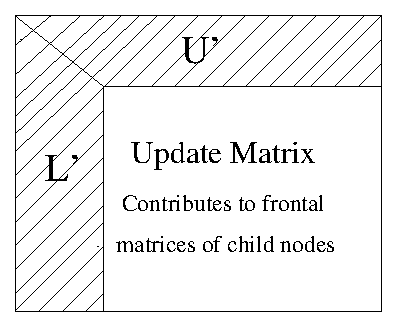
\includegraphics[width=0.25\textwidth]{figs/lu.eps}
\caption{A typical frontal matrix at a node of the DAG.}
\label{fig:lu}
\end{figure}

In Section~\ref{sec:parallel}, we looked at some of the benefits and
shortcomings of executing DAGs using the data- and demand-driven models. To
experimentally characterize the performance (speedup and memory footprint) of
these two models, we emulate the execution of a sparse unsymmetric-pattern
multifrontal algorithm for LU factorization with partial pivoting.  We choose
to emulate the LU factorization instead of implementing a real solver primarily
because while the effort required for such an implementation is 
huge~\footnote{There are only a handful of industrial strength codes for
unsymmetric sparse factorization, namely, MUMPS, PARDISO, SuperLU, UMFPACK, and
WSMP; details can be found in the survey by Gupta~\cite{GUPTAtoms01}.}, it is
easy to accurately capture the behavior of parallel execution time and memory
footprint by using the actual DAGs corresponding to real problems.  For our
emulation, we use the DAGs generated by the sparse solver in the Watson Sparse
Matrix Package (WSMP)~\cite{GUPTAsimax01,GUPTA00wsmp2}.

During its symbolic phase, Gupta's algorithm~\cite{GUPTAsimax01} generates a
task DAG $G =(E,V)$, where each vertex $v$ represents what is known as a
\textit{frontal matrix} in the parlance of multifrontal sparse
factorization~\cite{DUFF84siam} and the computation associated with it.  In the
data-DAG representation of this task DAG, an edge $e = (u \rightarrow{} v)$
symbolizes that $u$ produces data for $v$.  Alternately, in the demand-DAG
representation of this task DAG, an edge $e = (u \rightarrow{} v)$ symbolizes
that $u$ consumes data produced by $v$.  Figure~\ref{fig:lu} shows one such
frontal matrix at a vertex in the task DAG.  When a vertex in the task DAG is
executed, it performs a partial dense LU factorization on the frontal matrix
associated with that vertex, and the resulting \textit{update matrix} is used
by dependent vertices for filling their frontal matrices.  In the demand-driven
model, the memory required for the frontal matrix is allocated by the computing
vertex when it is ready to consume data from at least one of its completed
demand-children. In the data-driven model, as a task is spawned only after all
its data dependencies are satisfied, the memory required for the frontal matrix
is allocated upfront.  In both the data- and demand-driven models, the memory
allocated for the frontal matrix can only be deallocated when the data in the
update matrix has been consumed by all the dependent vertices (demand-parents
or data-children).

Our emulation begins by reading in the task DAG that encodes the weight of the
computation at each vertex and the data dependencies between vertices.  In the
WSMP solver, the data and the map for distribution of the update matrix at a
vertex among the frontal matrices of the dependent vertices are embedded pieces
of information.
% How does our implementation differ
Since our emulator does not have access to real data, it performs its
computations over simulated data values and distributes the update matrix
generated at each vertex equally among the vertex's dependent vertices.
Despite these two simplifying assumptions, our emulator generates a precise
speedup and memory profile of multifrontal sparse LU factorization.

Implementation of the data-driven model is straightforward and is akin to
Algorithm~\ref{alg:data}. In Section~\ref{sec:requirements}, we describe that
a tasking solution should support multiple notifications and continuations in
order to implement the demand-driven model. Being a new tasking library that is
under active development, PFunc currently lacks support for continuations. To
ensure deadlock-free execution under such conditions, we make use of PFunc's
support for task priorities and custom task scheduling. The deadlock scenario
described in Section~\ref{sec:cont} can be avoided if we disallow threads from
executing ancestor tasks while servicing descendants. For example, the deadlock
in Figure~\ref{fig:deadlock} can be avoided if we prevent thread $2$ from
picking task $D$ as it is still servicing task $F$, a descendant of task $D$.
To implement this strategy, we first traverse the demand-DAG in level-order (LO)
and number each vertex with its level. At the end of this exercise, each vertex
is numbered higher than any of its ancestors. These vertex LO numbers serve as
\textit{task priorities}.  Second, we enforce a scheduling policy that only
allows a thread $X$ which is servicing a task, say $A$, to pick a task, say $B$,
for execution when \code{priority}$(A) \le$ \code{priority}$(B)$.

\begin{figure}[t]
\centering
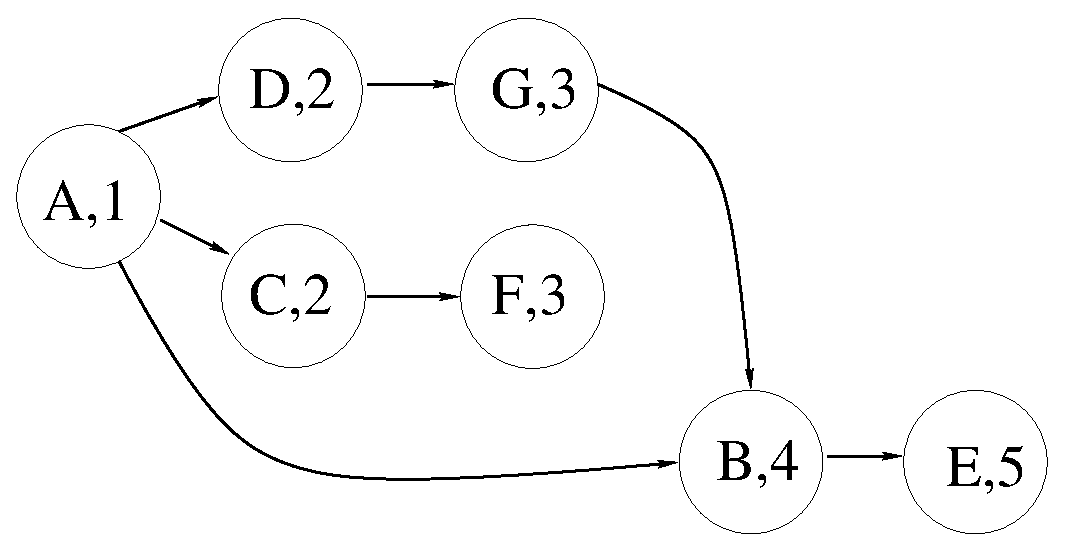
\includegraphics[width=0.35\textwidth]{figs/stealing.eps}
\caption{A demand-DAG that is parallelized with LO numbering.}
\label{fig:stealing}
\end{figure}

%
For example, consider the execution of the demand-DAG in
Figure~\ref{fig:stealing} where each node is depicted with its name (\code{A}
through \code{G}) and its LO number ($1$ through $5$). The LO number associated
with each node specifies its priority; the lower the number, the lower its
priority. To prevent deadlocks during the execution of this particular
demand-DAG, we need to ensure that a thread actively servicing task \code{B} or
task \code{E} must not pick task \code{D} or task \code{G}. As \code{D} and
\code{G} have lower priority than \code{B} and \code{E}, the scenario that can
lead to a deadlock is successfully avoided.

%
Using LO numbers coupled with prioritized scheduling has both advantages and
disadvantages. As we use the priorities to schedule tasks, we are able to
schedule critical tasks with higher priorities ahead of the non-critical tasks. 
%
However, using LO numbering with a custom task scheduling policy may constrict
parallelism by placing restrictions on the tasks that can be executed by a
thread.
%
Furthermore, to ensure that task priorities are respected during scheduling, we
make use of priority queues. Priority queues affect the performance in two
ways. First, in priority queues, insertion and removal of tasks takes longer
when compared to the \code{deque}s that are used many work-stealing tasking
models.  Second, by stipulating the owning and the stealing thread to operate
on different ends of the \code{deque}, using locks while operating on these
\code{deque}s is not always necessary~\cite{FrigoLeRa98}. However, in our
priority-based scheduling policy both the owning and the stealing thread
operate on the same end of the priority queue.  As a result, we lock the queue
for each and every each insertion and removal. This overhead, however,
is more than compensated for in the demand-driven execution with
recursive partitioning of the task DAG because the number of tasks 
created is relatively small compared to the data-driven execution.

% Thread Partitioning
In addition to the custom scheduling policy, we also employ a custom thread
partitioning strategy that allows us to turn task parallelism off when the
nodes perform very few computations. To achieve this goal, each node is
assigned a \textit{partition number} that regulates the execution of that node.
For example, if the partition number is one, the node has to execute all its
children and its own computations sequentially. The partition number of each
each node is determined by the cumulative weight of computations that are
performed by the sub-DAG rooted at that node. To save unnecessary task
creation overhead, when a node has relatively few computations to perform, it
is instructed to execute the sub-DAG rooted at it sequentially instead of
spawning new tasks.

% Data-driven implementations.
To benchmark the performance of the demand-driven model, we implemented the
data-driven model described in Algorithm~\ref{alg:data} using Cilk, OpenMP and
TBB.  The scheduling strategies implemented by both Cilk and TBB are similar
and, are described by Frigo et al~\cite{FrigoLeRa98}. OpenMP does not specify
the task scheduling policy to be used by its implementations.  However, as it
was heavily influenced by Cilk's tasking model~\cite{OmpTask}, it is reasonable
to assume that the scheduling policy is similar to that of Cilk.

In both the data- and demand-driven models, the per-node computations are
parallelized to maximize throughput. In the demand-driven model, the partition
number of a node is used as an upper limit bounding the data-parallelism in the
per-node computations. However, as there are no partition numbers associated
with the nodes in the data-driven model, the per-node computations are
parallelized using N, the total number of threads, as an upper limit bounding
the data parallelism. The data parallel portion uses smart block sizes to avoid
over parallelization of the per-node computations. This feature slightly
mitigates the effect of not knowing the partition number in the data-driven
model.  For example, if operating on a $50 \times 50$ matrix, even if $8$
threads were available, the computations are executed sequentially. 

\section{Experimental Results}
\label{sec:results}
In Section~\ref{sec:parallel}, we hypothesized that in certain applications,
the demand-driven execution scheme may be more advantageous than the
data-driven execution scheme.  To support this hypothesis, we present results
of running a sparse unsymmetric LU factorization emulation described in
Section~\ref{sec:lu} for a set of matrices from the University of Florida
Sparse Matrix Collection~\cite{davissparse}. Specifically, we benchmark the
memory consumption during the application run and the completion of the
execution.
%
The tests were run on an 8 core (two Intel Xeon x5365 quad-core) machine
running Linux 2.6.27.  For the Cilk implementation, we used the \code{Cilk
5.4.6} compiler.  The TBB implementation used the \code{GCC 4.3.2} compiler
with \code{TBB 2.1}.  PFunc implementation was also compiled with \code{GCC
4.3.2}. For the OpenMP implementation, we used \code{Sun CC} version
\code{5.10} as it has one of the better implementations of OpenMP tasks.

%
Memory consumption is a very important parameter of parallel execution.  When a
system consumes more memory than available, it either aborts or begins to swap
pages to disk, degrading performance significantly. Thus, it is highly
desirable that the maximum memory consumption during a particular run is
as small as possible.
%
Application runtime and memory consumption are both tightly coupled to the
scheduling algorithm of the execution environment. In order to get the best
application runtime, it is necessary to load balance the execution of the task
DAG. Similarly, scheduling producers and consumers such that the produced data
is quickly consumed and, their memory released is important in
minimizing the memory consumption during the application run.

Figures~\ref{memory_twotone} and~\ref{load_balance} show the memory
consumption and the per-thread workload during the execution of the matrix
\emph{twotone} with 8 threads.  As is evident, the threads share the workload
uniformly.  This is reflected in the execution of the demand-driven model which
is not only as fast as the data-driven model but also consumes significantly
less peak memory ($\approx 20\%$).
%
\insimgx{\columnwidth}{memory_twotone}{Memory consumption for \emph{twotone}
with 8 threads.}
%
\insimgx{\columnwidth}{load_balance}{Load distributions for \emph{twotone} and
\emph{g7jac200} with 8 threads for the TBB (data-driven) and PFunc
(demand-driven) implementations.}
% 
Figure~\ref{memory_g7jac200} shows another extreme with the
\emph{g7jac200} matrix where the demand-driven
execution takes significantly longer due to the lower parallelism (the deadlock
avoidance algorithm limits parallelism) than the data-driven execution.
Figure~\ref{load_balance} for \textit{g7jac200} clearly shows that the
threads execute vastly varying workloads in the demand-driven model.  However,
we also see that the peak memory consumption is significantly lower ($\approx
40\%$). If paging was triggered by such an execution, then it is very likely
that the demand-driven execution would finish faster.

\insimgx{\columnwidth}{memory_g7jac200}{Memory consumption for 
\emph{g7jac200} with 8 threads.}


Figure~\ref{dag_memory} shows the peak memory consumption of the
data- and demand-driven implementations with 8 threads relative to Cilk. 
%
\insimgx{\columnwidth}{dag_memory}{Peak memory consumption with 8 threads
relative to Cilk.}
%
We see that the memory consumption for the demand-driven execution is lower
than that of the data-driven implementations on average. 
%
Figure~\ref{dag_speedup} shows the application runtimes of the
data- and demand-driven implementations with 8 threads relative to Cilk. 
%
\insimgx{\columnwidth}{dag_speedup}{Performance with 8
threads relative to Cilk.}
%
%
We see that demand-driven execution performs comparably to other data-driven
execution schemes. The biggest outlier, the \emph{g7jac200} matrix, can be
explained by the imbalance in the execution DAG.  Some variance exists among
the data-driven model implementations due to the differences in the
implementations of the task parallel solutions themselves.
Figures~\ref{dag_memory} and~\ref{dag_speedup} allow us to conclude
that the demand-driven model shows promise to decrease the memory requirements
of sparse matrix factorization without losing performance in comparison to
the data-driven execution model. The lower memory consumption is due
to intelligent task scheduling enabled by the demand-driven model.

\section{Conclusions and Future Work}
\label{sec:conclusion}
As the number of cores per processor and the number of processors per socket
increase, programming models must minimize application memory footprints and
ensure good cache reuse. These are some of the strengths of the demand-driven
dataflow model. Our simulations have shown that the demand-driven model on
average consumes less memory while providing comparable performance to the
data-driven model for sparse unsymmetric LU factorizations. We have implemented
PFunc, a new library for task parallelism that allows realization of the
demand-driven dataflow model. In doing so, we have effectively identified key
requirements placed by the demand-driven model on task parallelism.

An important direction for future work is to implement CPS-style continuations
in PFunc so as to enable a more direct implementation of the demand-driven
model.  We believe that continuations in tandem with task priorities will allow
shorter runtimes and better memory profiles.  Finally, we plan to implement the
lessons learnt from this study back in the WSMP solver to improve its
performance.

\section{Acknowledgments}
\label{sec:ack}
We thank Jeremiah Willcock, Timo Schneider, Andrew Friedley and Laura Hopkins
for providing valuable insight that helped improve the quality of this paper.
This work was supported by IBM, National Science Foundation under grants
EIA-0202048 and EIA-0131354, and a grant from the Lilly Endowment.

\bibliographystyle{plain}
\bibliography{refs}

\end{document}
